% ============================================================
% Question Bank: ch02-04 Markups, Discounts, and Sales Tax
% Topic Title: Markups, Discounts, and Sales Tax
% CCSS: 7.RP.A.3
% Questions: 30 (18 MC + 7 SA + 5 Graphical)
% ============================================================

% --- Multiple Choice Questions (18) ---

\begin{practiceQuestion}{2-4-q01}{mc}
\begin{questionText}
A store buys a hat for $\$10$ and marks it up $80\%$. What is the selling price?
\end{questionText}
\choiceA{$\$8$}
\choiceB{$\$14$}
\choiceC{$\$18$}
\choiceD{$\$80$}
\correctAnswer{C}
\explanation{Markup: $10 \times 1.80 = \$18$.}
\end{practiceQuestion}

\begin{practiceQuestion}{2-4-q02}{mc}
\begin{questionText}
A $\$50$ backpack is $20\%$ off. What is the sale price?
\end{questionText}
\choiceA{$\$10$}
\choiceB{$\$30$}
\choiceC{$\$40$}
\choiceD{$\$45$}
\correctAnswer{C}
\explanation{$20\%$ off means you pay $80\%$: $50 \times 0.80 = \$40$.}
\end{practiceQuestion}

\begin{practiceQuestion}{2-4-q03}{mc}
\begin{questionText}
A meal costs $\$25$. Sales tax is $8\%$. What is the total cost?
\end{questionText}
\choiceA{$\$2$}
\choiceB{$\$23$}
\choiceC{$\$27$}
\choiceD{$\$33$}
\correctAnswer{C}
\explanation{Add tax: $25 \times 1.08 = \$27$.}
\end{practiceQuestion}

\begin{practiceQuestion}{2-4-q04}{mc}
\begin{questionText}
A store buys a lamp for $\$30$ and sells it for $\$48$. What is the percent markup?
\end{questionText}
\choiceA{$18\%$}
\choiceB{$37.5\%$}
\choiceC{$48\%$}
\choiceD{$60\%$}
\correctAnswer{D}
\explanation{Markup amount: $48 - 30 = 18$. Percent markup: $18 \div 30 = 0.60 = 60\%$.}
\end{practiceQuestion}

\begin{practiceQuestion}{2-4-q05}{mc}
\begin{questionText}
Shoes are on sale for $\$68$ after a $15\%$ discount. What was the original price?
\end{questionText}
\choiceA{$\$57.80$}
\choiceB{$\$78.20$}
\choiceC{$\$80$}
\choiceD{$\$83$}
\correctAnswer{C}
\explanation{After a $15\%$ discount the price is $85\%$ of original: $68 \div 0.85 = \$80$.}
\end{practiceQuestion}

\begin{practiceQuestion}{2-4-q06}{mc}
\begin{questionText}
A book costs $\$14$, and sales tax is $7\%$. What is the total?
\end{questionText}
\choiceA{$\$14.07$}
\choiceB{$\$14.70$}
\choiceC{$\$14.98$}
\choiceD{$\$15.40$}
\correctAnswer{C}
\explanation{Tax: $14 \times 0.07 = \$0.98$. Total: $14 + 0.98 = \$14.98$.}
\end{practiceQuestion}

\begin{practiceQuestion}{2-4-q07}{mc}
\begin{questionText}
A store buys jeans for $\$22$ and uses a $100\%$ markup. What is the selling price?
\end{questionText}
\choiceA{$\$22$}
\choiceB{$\$33$}
\choiceC{$\$44$}
\choiceD{$\$122$}
\correctAnswer{C}
\explanation{A $100\%$ markup doubles the cost: $22 \times 2.00 = \$44$.}
\end{practiceQuestion}

\begin{practiceQuestion}{2-4-q08}{mc}
\begin{questionText}
A $\$120$ jacket is $25\%$ off, and sales tax is $6\%$. What is the final price?
\end{questionText}
\choiceA{$\$85.20$}
\choiceB{$\$90.00$}
\choiceC{$\$93.60$}
\choiceD{$\$95.40$}
\correctAnswer{D}
\explanation{Discount: $120 \times 0.75 = \$90$. Tax: $90 \times 1.06 = \$95.40$.}
\end{practiceQuestion}

\begin{practiceQuestion}{2-4-q09}{mc}
\begin{questionText}
A toy store marks up a doll from $\$8$ to $\$14$. What is the percent markup?
\end{questionText}
\choiceA{$42.9\%$}
\choiceB{$57.1\%$}
\choiceC{$60\%$}
\choiceD{$75\%$}
\correctAnswer{D}
\explanation{Markup amount: $14 - 8 = 6$. Percent markup: $6 \div 8 = 0.75 = 75\%$.}
\end{practiceQuestion}

\begin{practiceQuestion}{2-4-q10}{mc}
\begin{questionText}
An online store charges $\$45$ for a sweater plus $9\%$ sales tax. What is the total?
\end{questionText}
\choiceA{$\$45.09$}
\choiceB{$\$45.90$}
\choiceC{$\$49.05$}
\choiceD{$\$54$}
\correctAnswer{C}
\explanation{$45 \times 1.09 = \$49.05$.}
\end{practiceQuestion}

\begin{practiceQuestion}{2-4-q11}{mc}
\begin{questionText}
A $\$200$ television is discounted $30\%$. Then the store applies $5\%$ sales tax. What is the final price?
\end{questionText}
\choiceA{$\$130$}
\choiceB{$\$133$}
\choiceC{$\$140$}
\choiceD{$\$147$}
\correctAnswer{D}
\explanation{Discount: $200 \times 0.70 = \$140$. Tax: $140 \times 1.05 = \$147$.}
\end{practiceQuestion}

\begin{practiceQuestion}{2-4-q12}{mc}
\begin{questionText}
A store buys a watch for $\$45$, marks it up $40\%$, then offers the customer $10\%$ off. What is the final selling price before tax?
\end{questionText}
\choiceA{$\$54.00$}
\choiceB{$\$56.70$}
\choiceC{$\$58.50$}
\choiceD{$\$63.00$}
\correctAnswer{B}
\explanation{Markup: $45 \times 1.40 = \$63$. Discount: $63 \times 0.90 = \$56.70$.}
\end{practiceQuestion}

\begin{practiceQuestion}{2-4-q13}{mc}
\begin{questionText}
Which is the correct order to calculate a final price?
\end{questionText}
\choiceA{Tax → Discount → Markup}
\choiceB{Markup → Tax → Discount}
\choiceC{Discount → Tax → Markup}
\choiceD{Markup → Discount → Tax}
\correctAnswer{D}
\explanation{Apply markup first (store sets price), then discount (sale), then tax (at checkout). Tax is always last.}
\end{practiceQuestion}

\begin{practiceQuestion}{2-4-q14}{mc}
\begin{questionText}
A phone costs $\$350$ after a $30\%$ markup. What did the store pay for the phone?
\end{questionText}
\choiceA{$\$245$}
\choiceB{$\$269.23$}
\choiceC{$\$280$}
\choiceD{$\$320$}
\correctAnswer{B}
\explanation{After a $30\%$ markup, selling price $= 1.30 \times \text{cost}$. Cost $= 350 \div 1.30 \approx \$269.23$.}
\end{practiceQuestion}

\begin{practiceQuestion}{2-4-q15}{mc}
\begin{questionText}
A $\$60$ video game is on sale for $15\%$ off. Sales tax is $7\%$. What is the total cost?
\end{questionText}
\choiceA{$\$48.42$}
\choiceB{$\$51.00$}
\choiceC{$\$54.57$}
\choiceD{$\$55.47$}
\correctAnswer{C}
\explanation{Discount: $60 \times 0.85 = \$51$. Tax: $51 \times 1.07 = \$54.57$.}
\end{practiceQuestion}

\begin{practiceQuestion}{2-4-q16}{mc}
\begin{questionText}
A bakery buys flour for $\$5$ per bag and sells muffins made from one bag for $\$20$. What is the percent markup on the flour cost?
\end{questionText}
\choiceA{$75\%$}
\choiceB{$150\%$}
\choiceC{$200\%$}
\choiceD{$300\%$}
\correctAnswer{D}
\explanation{Markup amount: $20 - 5 = 15$. Percent markup: $15 \div 5 = 3.00 = 300\%$.}
\end{practiceQuestion}

\begin{practiceQuestion}{2-4-q17}{mc}
\begin{questionText}
A coat originally costs $\$85$. It goes on clearance for $40\%$ off, then an additional $10\%$ off the sale price. What is the final price before tax?
\end{questionText}
\choiceA{$\$42.50$}
\choiceB{$\$45.90$}
\choiceC{$\$51.00$}
\choiceD{$\$55.25$}
\correctAnswer{B}
\explanation{First discount: $85 \times 0.60 = \$51$. Second discount: $51 \times 0.90 = \$45.90$.}
\end{practiceQuestion}

\begin{practiceQuestion}{2-4-q18}{mc}
\begin{questionText}
Two stores sell the same $\$80$ headphones. Store A offers $25\%$ off. Store B offers $\$20$ off. Which is a better deal?
\end{questionText}
\choiceA{Store A (you pay $\$55$)}
\choiceB{Store B (you pay $\$55$)}
\choiceC{Store A (you pay $\$60$)}
\choiceD{Both stores give the same price}
\correctAnswer{D}
\explanation{Store A: $80 \times 0.75 = \$60$. Store B: $80 - 20 = \$60$. Both give the same price of $\$60$.}
\end{practiceQuestion}

% --- Short Answer Questions (7) ---

\begin{practiceQuestion}{2-4-q19}{sa}
\begin{questionText}
A store buys a board game for $\$16$ and marks it up $125\%$. What is the selling price?
\end{questionText}
\correctAnswer{$\$36$}
\explanation{$16 \times 2.25 = \$36$.}
\end{practiceQuestion}

\begin{practiceQuestion}{2-4-q20}{sa}
\begin{questionText}
A $\$72$ pair of sneakers is $35\%$ off. What is the sale price?
\end{questionText}
\correctAnswer{$\$46.80$}
\explanation{$72 \times 0.65 = \$46.80$.}
\end{practiceQuestion}

\begin{practiceQuestion}{2-4-q21}{sa}
\begin{questionText}
A restaurant bill is $\$32$. Sales tax is $6.5\%$. What is the total?
\end{questionText}
\correctAnswer{$\$34.08$}
\explanation{$32 \times 1.065 = \$34.08$.}
\end{practiceQuestion}

\begin{practiceQuestion}{2-4-q22}{sa}
\begin{questionText}
A store buys a skateboard for $\$35$ and sells it for $\$56$. What is the percent markup?
\end{questionText}
\correctAnswer{$60\%$}
\explanation{Markup: $56 - 35 = 21$. Percent: $21 \div 35 = 0.60 = 60\%$.}
\end{practiceQuestion}

\begin{practiceQuestion}{2-4-q23}{sa}
\begin{questionText}
A laptop is on sale for $\$680$ after a $15\%$ discount. What was the original price?
\end{questionText}
\correctAnswer{$\$800$}
\explanation{$680 \div 0.85 = \$800$.}
\end{practiceQuestion}

\begin{practiceQuestion}{2-4-q24}{sa}
\begin{questionText}
Concert tickets cost $\$55$ each. There is a $12\%$ service fee and $8\%$ sales tax on the ticket-plus-fee total. What is the total cost of one ticket?
\end{questionText}
\correctAnswer{$\$66.53$}
\explanation{Fee: $55 \times 1.12 = \$61.60$. Tax: $61.60 \times 1.08 = \$66.528 \approx \$66.53$.}
\end{practiceQuestion}

\begin{practiceQuestion}{2-4-q25}{sa}
\begin{questionText}
A $\$40$ shirt has a $10\%$ discount, then $7\%$ sales tax. What is the final price?
\end{questionText}
\correctAnswer{$\$38.52$}
\explanation{Discount: $40 \times 0.90 = \$36$. Tax: $36 \times 1.07 = \$38.52$.}
\end{practiceQuestion}

% --- Graphical Questions (3 GMC + 2 GSA) ---

\begin{practiceQuestion}{2-4-q26}{gmc}
\begin{questionText}
The diagram shows the steps to find the final price of an item. What is the final price?

\begin{center}
\begin{tikzpicture}[scale=0.8, every node/.style={font=\small}]
  \node[draw,rounded corners,fill=funBlue!20,minimum width=2cm] (cost) at (0,0) {Cost: $\$40$};
  \node[draw,rounded corners,fill=funGreen!20,minimum width=2cm] (markup) at (4,0) {$+50\%$ markup};
  \node[draw,rounded corners,fill=funOrange!20,minimum width=2cm] (discount) at (8,0) {$-20\%$ discount};
  \node[draw,rounded corners,fill=funRed!20,minimum width=2cm] (tax) at (12,0) {$+10\%$ tax};
  \draw[thick,->] (cost) -- (markup);
  \draw[thick,->] (markup) -- (discount);
  \draw[thick,->] (discount) -- (tax);
\end{tikzpicture}
\end{center}
\end{questionText}
\choiceA{$\$48.00$}
\choiceB{$\$50.40$}
\choiceC{$\$52.80$}
\choiceD{$\$56.00$}
\correctAnswer{C}
\explanation{Markup: $40 \times 1.50 = \$60$. Discount: $60 \times 0.80 = \$48$. Tax: $48 \times 1.10 = \$52.80$.}
\end{practiceQuestion}

\begin{practiceQuestion}{2-4-q27}{gmc}
\begin{questionText}
The table shows the cost and selling price of four items. Which item has the greatest percent markup?

\begin{center}
\begin{tabular}{|l|c|c|}
\hline
\textbf{Item} & \textbf{Cost} & \textbf{Selling Price} \\
\hline
Hat & $\$8$ & $\$14$ \\
\hline
Scarf & $\$12$ & $\$18$ \\
\hline
Gloves & $\$6$ & $\$12$ \\
\hline
Belt & $\$15$ & $\$24$ \\
\hline
\end{tabular}
\end{center}
\end{questionText}
\choiceA{Hat}
\choiceB{Scarf}
\choiceC{Gloves}
\choiceD{Belt}
\correctAnswer{C}
\explanation{Hat: $(14-8)/8 = 75\%$. Scarf: $(18-12)/12 = 50\%$. Gloves: $(12-6)/6 = 100\%$. Belt: $(24-15)/15 = 60\%$. Gloves has the greatest markup at $100\%$.}
\end{practiceQuestion}

\begin{practiceQuestion}{2-4-q28}{gmc}
\begin{questionText}
The bar model below shows the breakdown of a customer's total payment. What was the original price of the item before the sales tax?

\begin{center}
\begin{tikzpicture}[scale=0.65]
  \fill[funBlue!40] (0,0) rectangle (9,1);
  \fill[funRed!40] (9,0) rectangle (10,1);
  \draw[thick] (0,0) rectangle (10,1);
  \draw[thick] (9,0) -- (9,1);
  \node[font=\small] at (4.5,0.5) {Original price};
  \node[font=\small] at (9.5,0.5) {Tax};
  \draw[thick,<->] (0,-0.4) -- (10,-0.4) node[midway,below,font=\small] {Total $= \$53.50$};
  \node[above,font=\small] at (9.5,1) {$7\%$};
\end{tikzpicture}
\end{center}
\end{questionText}
\choiceA{$\$46.76$}
\choiceB{$\$49.76$}
\choiceC{$\$50.00$}
\choiceD{$\$52.00$}
\correctAnswer{C}
\explanation{The total is $1.07$ times the original. Original $= 53.50 \div 1.07 = \$50.00$.}
\end{practiceQuestion}

\begin{practiceQuestion}{2-4-q29}{gsa}
\begin{questionText}
The receipt below shows a purchase. Find the missing sales tax amount.

\begin{center}
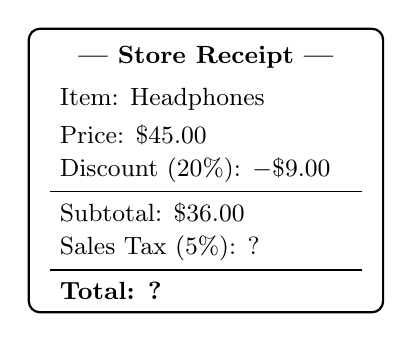
\begin{tikzpicture}[scale=0.9]
  \draw[thick,rounded corners] (0,0) rectangle (5,4);
  \node[font=\small\bfseries] at (2.5,3.6) {--- Store Receipt ---};
  \node[anchor=west,font=\small] at (0.3,3.0) {Item: Headphones};
  \node[anchor=west,font=\small] at (0.3,2.5) {Price: $\$45.00$};
  \node[anchor=west,font=\small] at (0.3,2.0) {Discount (20\%): $-\$9.00$};
  \draw[thin] (0.3,1.7) -- (4.7,1.7);
  \node[anchor=west,font=\small] at (0.3,1.4) {Subtotal: $\$36.00$};
  \node[anchor=west,font=\small] at (0.3,0.9) {Sales Tax (5\%): ?};
  \draw[thick] (0.3,0.6) -- (4.7,0.6);
  \node[anchor=west,font=\small\bfseries] at (0.3,0.3) {Total: ?};
\end{tikzpicture}
\end{center}

What is the sales tax amount and the total?
\end{questionText}
\correctAnswer{Tax $= \$1.80$; Total $= \$37.80$}
\explanation{Tax on subtotal: $36.00 \times 0.05 = \$1.80$. Total: $36.00 + 1.80 = \$37.80$.}
\end{practiceQuestion}

\begin{practiceQuestion}{2-4-q30}{gsa}
\begin{questionText}
A store buys and sells the items shown in the table. What is the total profit (markup amount) the store makes on selling one of each item?

\begin{center}
\begin{tabular}{|l|c|c|}
\hline
\textbf{Item} & \textbf{Cost to Store} & \textbf{Markup} \\
\hline
Water bottle & $\$4$ & $50\%$ \\
\hline
Notebook & $\$3$ & $100\%$ \\
\hline
Pen set & $\$5$ & $60\%$ \\
\hline
\end{tabular}
\end{center}
\end{questionText}
\correctAnswer{$\$8$}
\explanation{Water bottle markup: $4 \times 0.50 = \$2$. Notebook markup: $3 \times 1.00 = \$3$. Pen set markup: $5 \times 0.60 = \$3$. Total profit: $2 + 3 + 3 = \$8$.}
\end{practiceQuestion}
